\subsubsection{Primer 3 - Šifrovana komunikacija}

\large{1. Opis zadatka}
\normalsize

Napraviti Client-Server aplikaciju koja će komunicirati na TCP portu X (gde je $X = broj\ indeksa/24 + 2000$) i omogućavati klijentima šifrovanu komunikaciju koristeći Vigenere tablu sa ključem.

\large{2. Opis šifrovanja}
\normalsize

Vigenere tabla se koristi u šifrovanju poruka pomoću Vigenere šifre. Sastoji se od kvadratne tabele sa 26 redova i 26 kolona, gde svaki red sadrži slova engleskog alfabeta pomerenog za jedno mesto u odnosu na prethodni red. Vigenere tabla sa ključem dodaje kompleksnost tako što se u prvom redu prvo stavljaju sva slova iz ključa, pa tek ostatat alfabeta bez tih slova. 

Da biste šifrovali poruku, prvo odaberete ključnu reč koja se ponavlja do dužine originalne poruke. Ukoliko je ključna reč kraća od originalne poruke, ključna reč se ponavlja sve dok ne dostigne dužinu originalne poruke (Ingorisaći bele i specijalne karaktere), a ukoliko je duža od originalne poruke onda se preseca. Svako slovo u poruci se zatim šifruje kombinovanjem sa odgovarajućim slovom ključne reči korišćenjem tabele: pronađete red koji odgovara slovu ključne reči i kolonu koja odgovara slovu originalne poruke. Slovo na preseku reda i kolone je šifrovano slovo. Dekodiranje se vrši obrnutim procesom koristeći istu tabelu i ključnu reč.

\begin{figure}[H]
    \centering
    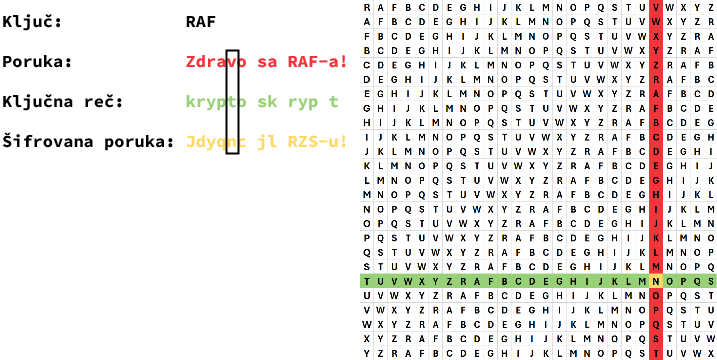
\includegraphics[width=0.85\textwidth]{Slike/VTB/VTB_Sifrovanje.png}
    \caption*{Primer šifrovanja koristeći Vigenere tabelu sa ključem "RAF"}
    \label{fig:vtb_primer}
\end{figure}

\large{3. Specifikacija zadatka}
\normalsize

Aplikacija treba da podrži konekciju \textbf{maksimalno} 2 klijenta. Nakon početka aplikacije, komunikacija kreće tek kada oba igrača kažu start. Pri početku, klijent 1 klijentu 2 šalje ključ i ključnu reč. Oba klijenta generišu alpfabet prema ključu i svu dalju enkripciju i dekripciju rade prema generisanoj Vigenere tabeli i ključnoj reči. Klijent 1 sada šalje poruku klijentu 2. Klijent 2 dešifruje i ispisuje poruku, nakon čega uzvraća šifrovanu poruku. Komunikacija se obavlja sve dok jedan od klijenata ne napiše "!KRAJ!".

\begin{figure}[H]
    \centering
    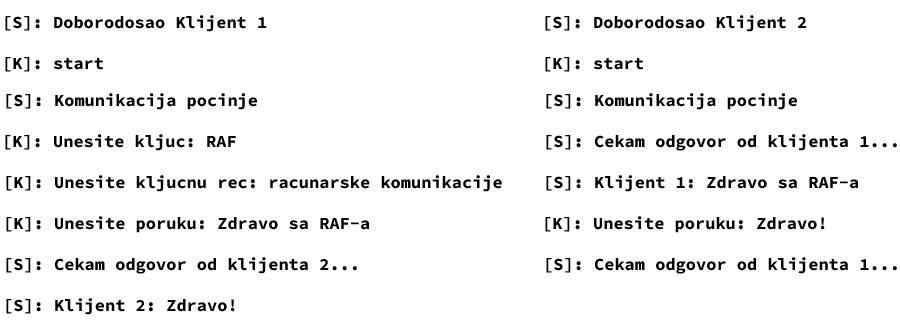
\includegraphics[width=0.85\textwidth]{Slike/VTB/VTB_Primer_komunikacije.png}
    \caption*{Primer komunikacije}
    \label{fig:vtb_primer_komunikacije}
\end{figure}